\documentclass[10pt,a4paper]{article}
\usepackage[utf8]{inputenc}
\usepackage{amsmath}
\usepackage{gensymb}
\usepackage{amsfonts}
\usepackage{siunitx}
\usepackage[european]{circuitikz}
\usepackage{geometry}
\newgeometry{tmargin=2cm, bmargin=2cm, lmargin=2cm, rmargin=2cm}
\usepackage{amssymb}
\usepackage{polski}
\usepackage{graphicx}
\author{\textbf{T. Fąs}}
\title{\textbf{WYZNACZANIE STAŁEJ STEFANA-BOLTZMANNA}}
\begin{document}
\maketitle

\begin{center}
\textbf{\subsection*{STRESZCZENIE}}
\end{center}
Wyznaczona wartość stałej Stefana-Boltzmanna wynosi $\sigma=(2,51\pm0,56)\cdot 10^{-8}$ W/m$^2$K$^4$. Otrzymana wartość jest dwukrotnie niższa od wartości teoretycznej, najprawdopodobniej na skutek błędów aparatury pomiarowej.
\begin{center}
\textbf{\subsection*{WSTĘP}}
\end{center}
Ciało doskonale czarne to obiekt, który pochłania całe promieniowanie jakie nań pada.
Prawo Stefana-Boltzmanna przedstawiające całkowitą moc emitowaną przez to ciało, wyraża się wzorem:
\begin{equation}
 W(T)=\sigma S T^4,
 \end{equation} 
 gdzie $T$ jest temperaturą ciała wyrażoną w kelwinach, $S$ jest polem powierzchni ciała, a $\sigma$ to stała Stefana-Boltzmanna.
Każde rzeczywiste ciało ma skuteczność emisji $\epsilon$ mniejszą od ciała doskonale czarnego, dodatkowo należy uwzględnić temperaturę otoczenia $T_{0}$. Różnica emitowanej mocy między ciałem doskonale czarnym, a każdym innym, o takim samym polu powierzchni $S$ wyraża się wzorem:
\begin{equation}
\Delta W=(1-\epsilon)S\sigma(T^4-T_{0}^4)
\end{equation}
Celem doświadczenia było zmierzenie tej różnicy dla walca okopconego, który imitował ciało doskonale czarne i dla walca srebrnego o identycznych polach powierzchni. Znając wartości $\Delta W$, $\epsilon$ i $S$ można wyznaczyć wartość stałej Stefana-Boltzmanna
\begin{center}
\textbf{\subsection*{UKŁAD DOŚWIADCZALNY}}
\end{center}
Układ doświadczalny składał się z walca okopconego i srebrzystego (wypolerowanego), o identycznych rozmiarach, dwóch mierników CHY 38, dwóch grzałek o identycznych oporach, zasilacza, termopar miedź-konstantan, miski z lodem oraz z mikrowoltomierza NI-9211. Schemat układu został przedstawiony na Rysunku 1.

\begin{figure}[h!]
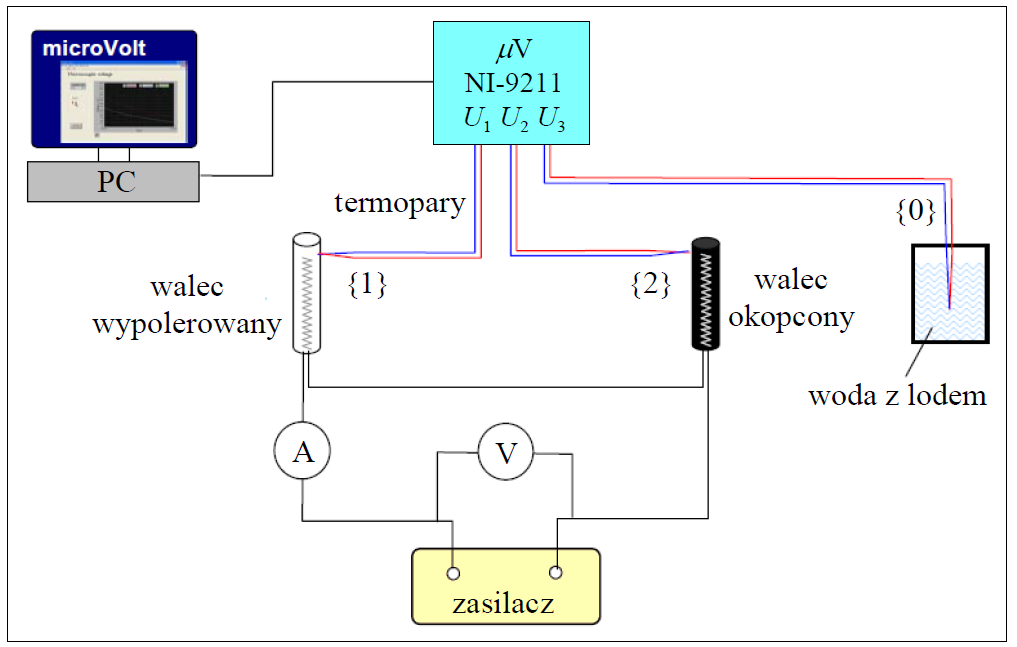
\includegraphics[width=15cm]{rap11ukl} 
\centering
\caption{Układ pomiarowy.}
\end{figure}

 Mierniki CHY zostały wykorzystane w charakterze woltomierza i amperomierza. Pozwoliło to na wyznaczenie mocy grzałek. Mikrowoltomierz dokonywał pomiaru napięcia na termoparach podłączonych do walców, co pozwoliło na pomiar temperatury walców. Jedna z termopar była zanurzona w misce z wodą z lodem, która służyła jako punkt odniesienia pomiaru temperatur. Dzięki pomiarom temperatury można było otrzymać zależność mocy od temperatury dla każdego z walców. Różnica tych funkcji pozwoliłaby na wyznaczenie stałej Stefana-Boltzmanna z Równania (2). 
\begin{center}
\textbf{\subsection*{WYNIKI POMIARÓW}}
\end{center}
Pomiary przeprowadzono dla czterech rożnych wartości napięcia. Wartości te przedstawiono w Tabeli 1. Na samym początku wykonano też jeden pomiar bez grzania. Ilość punktów pomiarowych związana z tymi pomiarami jest zbyt duża, by umieszczać je w raporcie.
\begin{table}[h!]
\centering
\caption{Napięcia, natężenia i ich niepewności}
\begin{tabular}{|c|c|c|c|c|c|}
\hline
Pomiar           & 1      & 2      & 3      & 4            \\ \hline
Napięcie $U$ [V]   & 12,05   & 17,02   & 22,0   & 27,0     \\ \hline
Natężenie $I$ [A]  & 0,60 & 0,85 & 1,10 & 1,35  \\ \hline
Niepewność $U$ [V] & 0,070   & 0,095 & 0,21 & 0,24  \\ \hline
Niepewność $I$ [A] & 0,028 & 0,036 &0,043 & 0,051  \\ \hline
\end{tabular}
\end{table}
Przy pomocy suwmiarki dokonano pomiarów średnicy i wysokości walców. Jako, że eksperyment zakłada identyczność walców, to dane te, Znajdujące się w Tabeli 2, będą traktowane jako pochodzące od jednego walca.

\begin{table}[h!]
\centering
\caption{Wymiary walców.}
\begin{tabular}{|c|c|c|c|c|c|}
\hline
Średnica D [mm] & 12,0        & 12,0        & 12,0    & 11,9   & 12,0   \\ \hline
Wysokość H [mm] & \multicolumn{2}{c|}{84,3} & \multicolumn{3}{c|}{85,2} \\ \hline
\end{tabular}
\end{table}

\begin{center}
\textbf{\subsection*{ANALIZA DANYCH}}
\end{center}
W pierwszej kolejności wykonano wykres związany z napięciami przy wyłączonej grzałce. Jest on pokazany na Rysunku 2. Niepewności $u$ związanie z pomiarem napięć $V$ na mikrowoltomierzu obliczono, korzystając ze wzoru:
\begin{equation}
u_{\mu V}=0,001\cdot V+5 \, \mu V,
\end{equation}

\begin{figure}[h!]
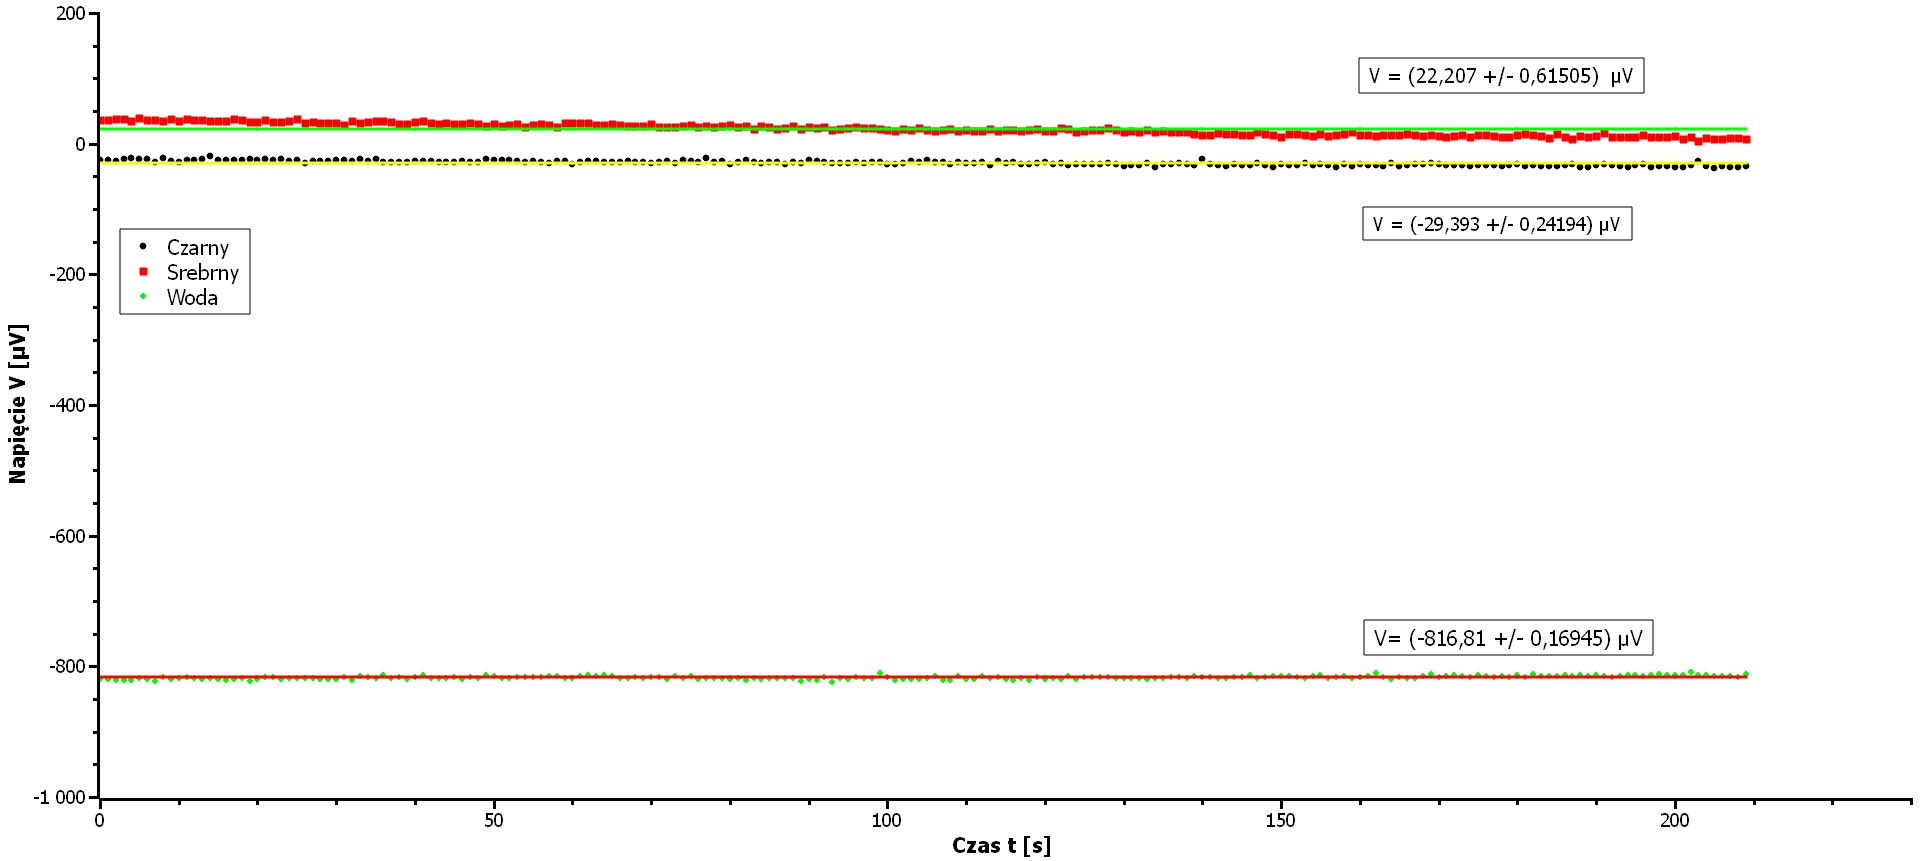
\includegraphics[width=15cm]{rap11rys1} 
\centering
\caption{Napięcia bez grzania}
\end{figure}

Korzystając z wartości dopasowano do obu walców funkcje stałe, które są tożsame z ich temperaturą pokojową. 

Zależność temperatury od napięcia podana przez producenta termopar dana jest wzorem:
\begin{equation}
T(V)=a+b(V-V_{0})+c(V-V_{0})^2,
\end{equation}
gdzie $a=1,75 \, ^{\circ}$C, $b=0,02385\, ^{\circ}$C/$\mu V$ oraz $c=-2,6072\cdot10^{-7}\, ^{\circ}$C/$\mu V^2$. Niepewność związana z temperaturą dana jest wzorem;
\begin{equation}
\Delta_{T}=0,5\%\cdot T+0,5^{\circ}C
\end{equation}

Aby wyznaczyć wartość $V_{0}$ z Równania (4) podstawiono za $V$ wartość $V=-816,81$ $\mu$V, gdyż założono, że temperatura wody z lodem wynosi $0 \,^{\circ}$C. Otrzymano dwie wartość, z których wybrano tę, która dawała dodatnie wartości temperatury dla napięć walców. Otrzymano $V_{0}=-743,493$ $\mu$V. 

Temperatury walców otrzymano, podstawiając wartości ich napięć do Równania (4). Założono, że w chwili początkowej ich temperatury były równe, więc postanowiono uśrednić wartości ich temperatur. Skorzystano ze średnie ważonej, posługując się odwrotnościami niepewności temperatur z Równania (5) jako wagami. Otrzymano $T_{0}=(19,25\pm0,42) \,^{\circ}$C. Za niepewność przyjęto większą z niepewności wewnętrznej i zewnętrznej.
Niepewności $u$ dla mierników CHY 38, związanych z pomiarami napięcia $U$ i natężenia $I$ obliczono z następujących wzorów:
\begin{equation}
u_{U}=0,005\cdot U+0,01 \, V
\end{equation}
\begin{equation}
u_{I}=0,03\cdot I+0,01 \, A
\end{equation}
Wartości niepewności $u_{U}$ i $u_{I}$ zostały umieszczone w Tabeli 1.

Napięcie $V$ na termoparach jest dane funkcją:
\begin{equation}
V(t)=V_{\infty}-V_{0}\exp(-\lambda t)
\end{equation}
gdzie $V_{\infty}$, $V_{0}$ i $\lambda$ są parametrami dopasowania. Dla bardzo długiego czasu wartość eksponensu dąży do zera, więc dominującym czynnikiem staje się $V_{\infty}$. Jest to szukana wartość napięcia w stanie stacjonarnym. 

W celu dopasowania krzywej do punktów pomiarowych wykorzystano program Gnuplot. Niepewności pomiarów obliczono z Równania (3) i uwzględniono je w analizie. Wyniki dopasowań dla pomiaru pierwszego przedstawione są na Rysunku 3.
Wszystkie krzywe przechodzą test $\chi^2$, ponieważ dla takiej liczby punktów pomiarowych wartości krytyczne $\chi^2$ są rzędu $10^3$. 
 
Analogiczne wykresy dla kolejnych pomiarów są przedstawione na Rysunkach 4-6.

\begin{figure}[h!]
\centering
\begin{minipage}{0.5\textwidth}
  \centering
  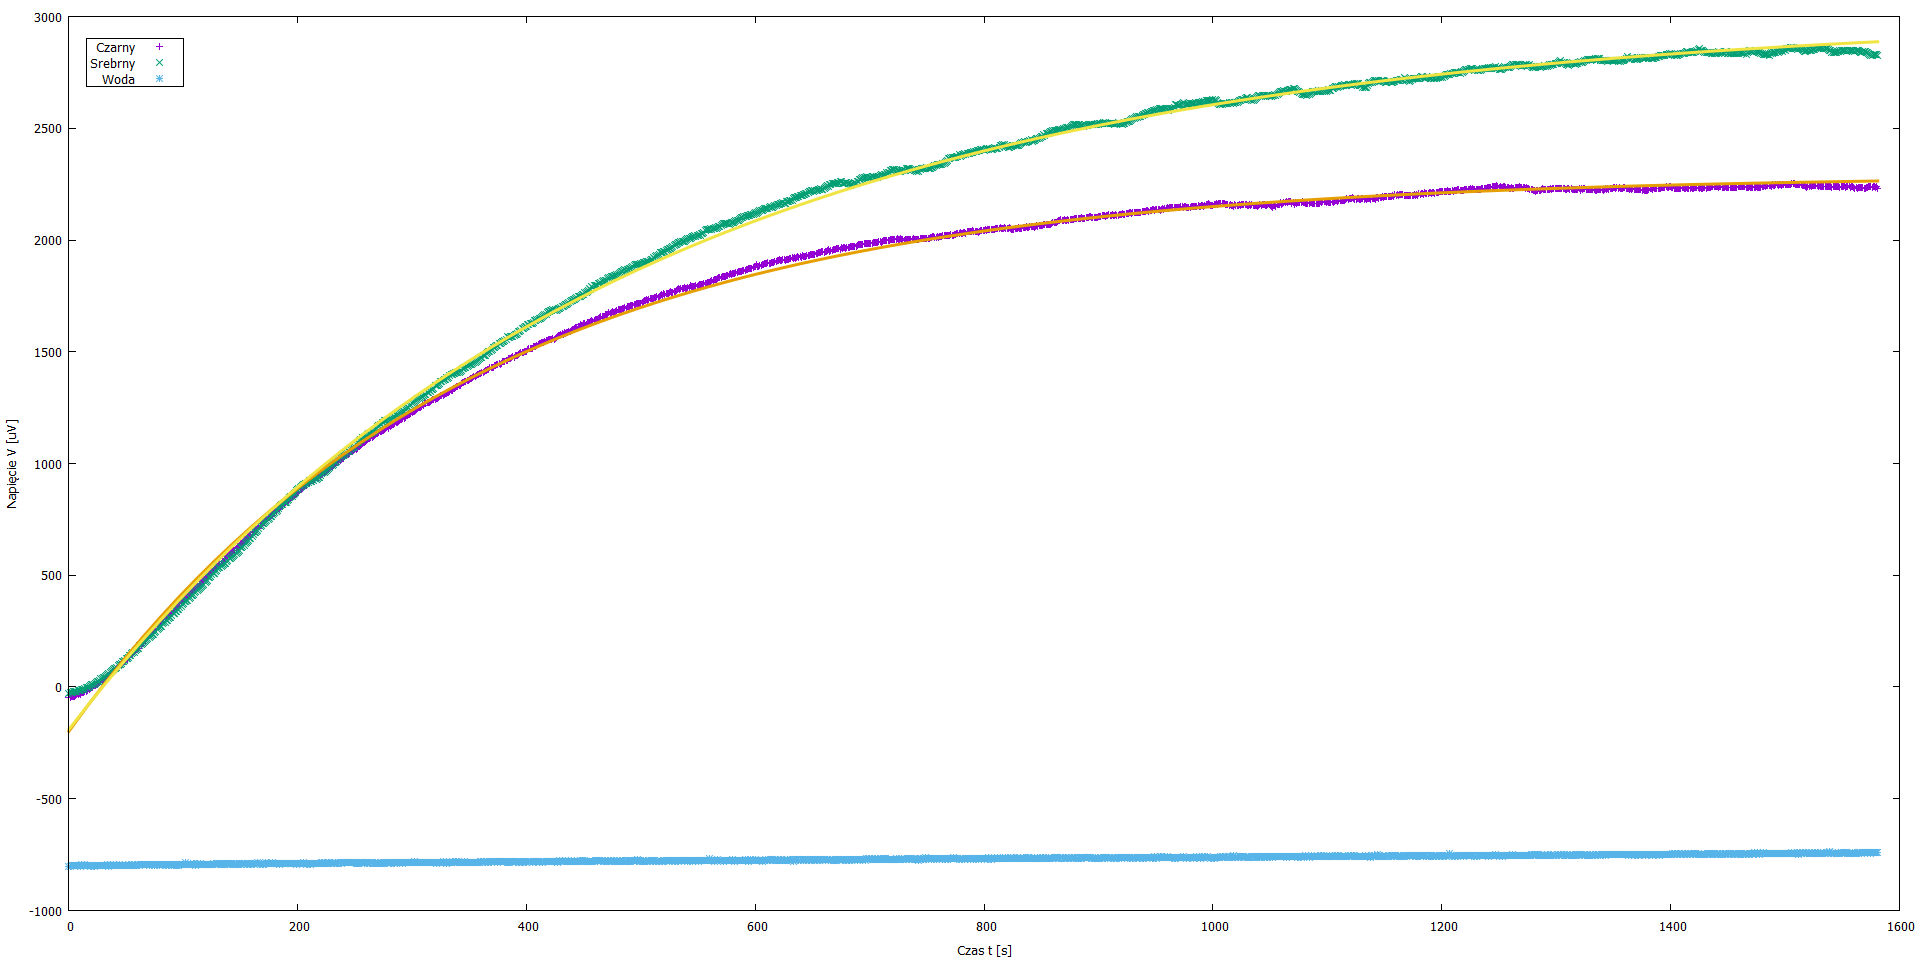
\includegraphics[width=8cm, height=5cm ]{rap11rys2} 
\caption{Dopasowanie krzywej: pomiar 1.}
\end{minipage}%
\begin{minipage}{0.5\textwidth}
  \centering
  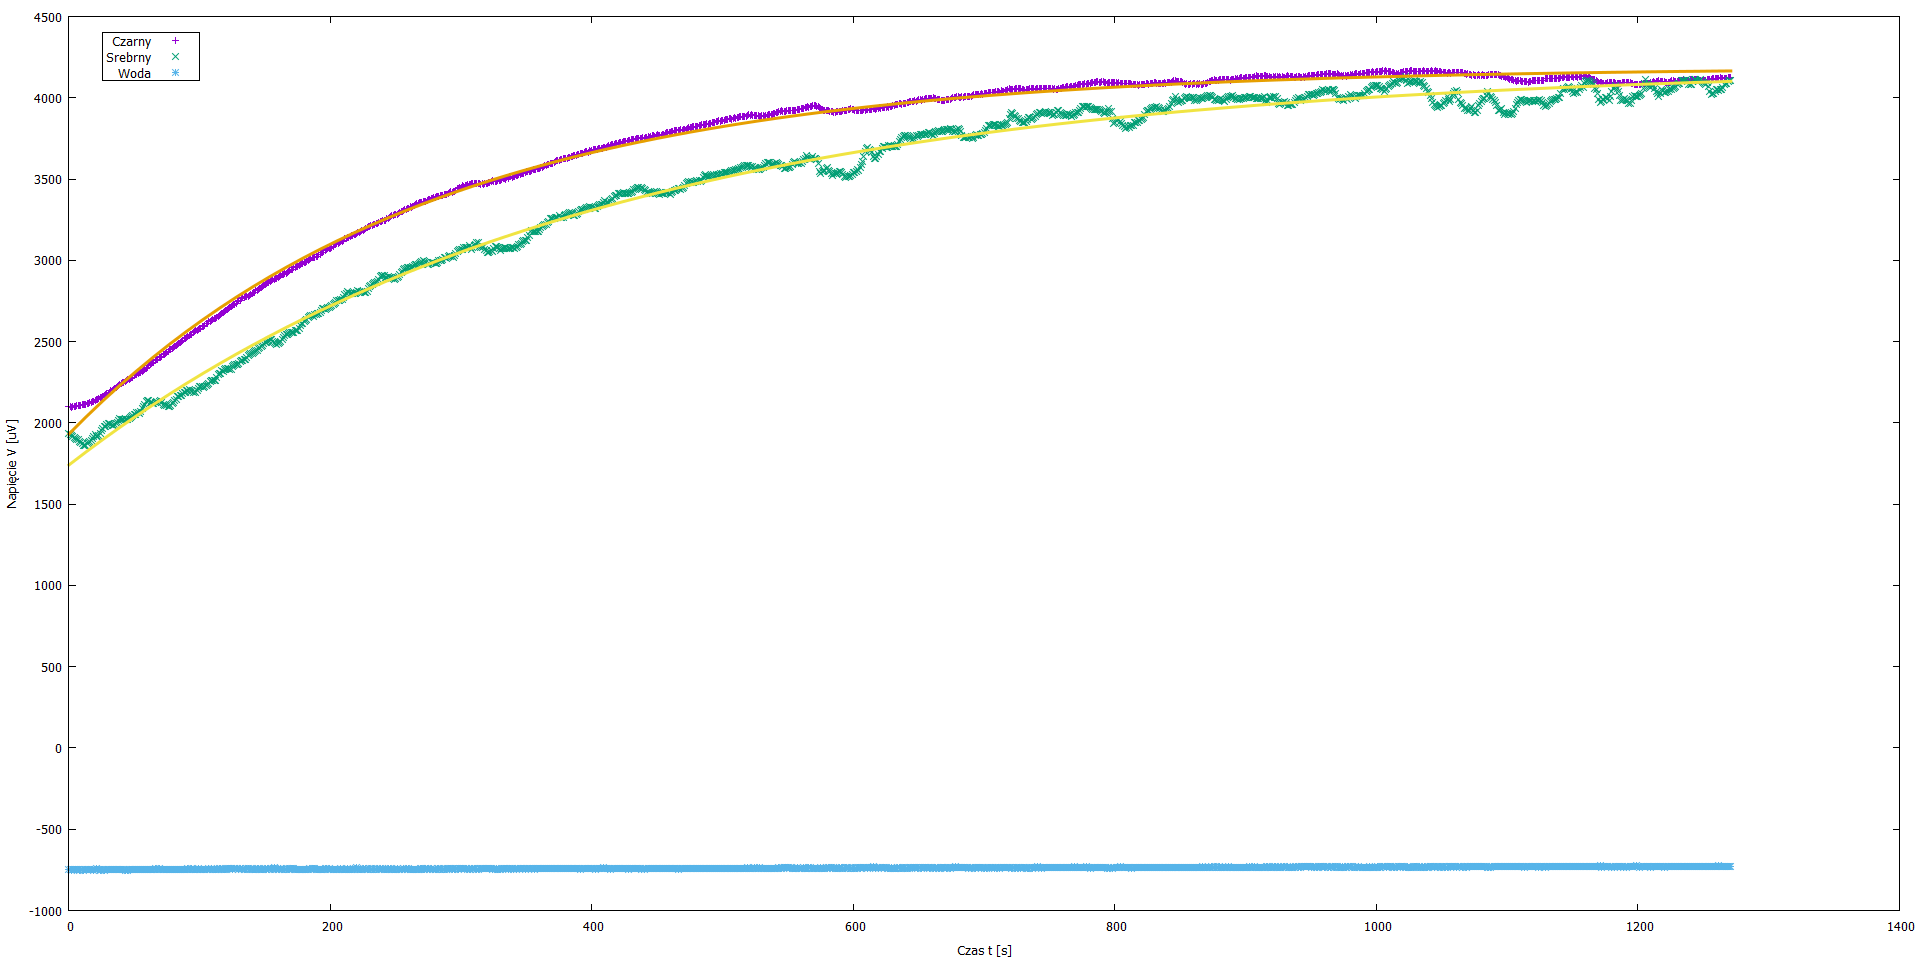
\includegraphics[width=8cm, height=5cm ]{rap11rys3} 
\caption{Dopasowanie krzywej: pomiar 2.}
\end{minipage}
\end{figure}

\begin{figure}[h!]
\centering
\begin{minipage}{0.5\textwidth}
  \centering
  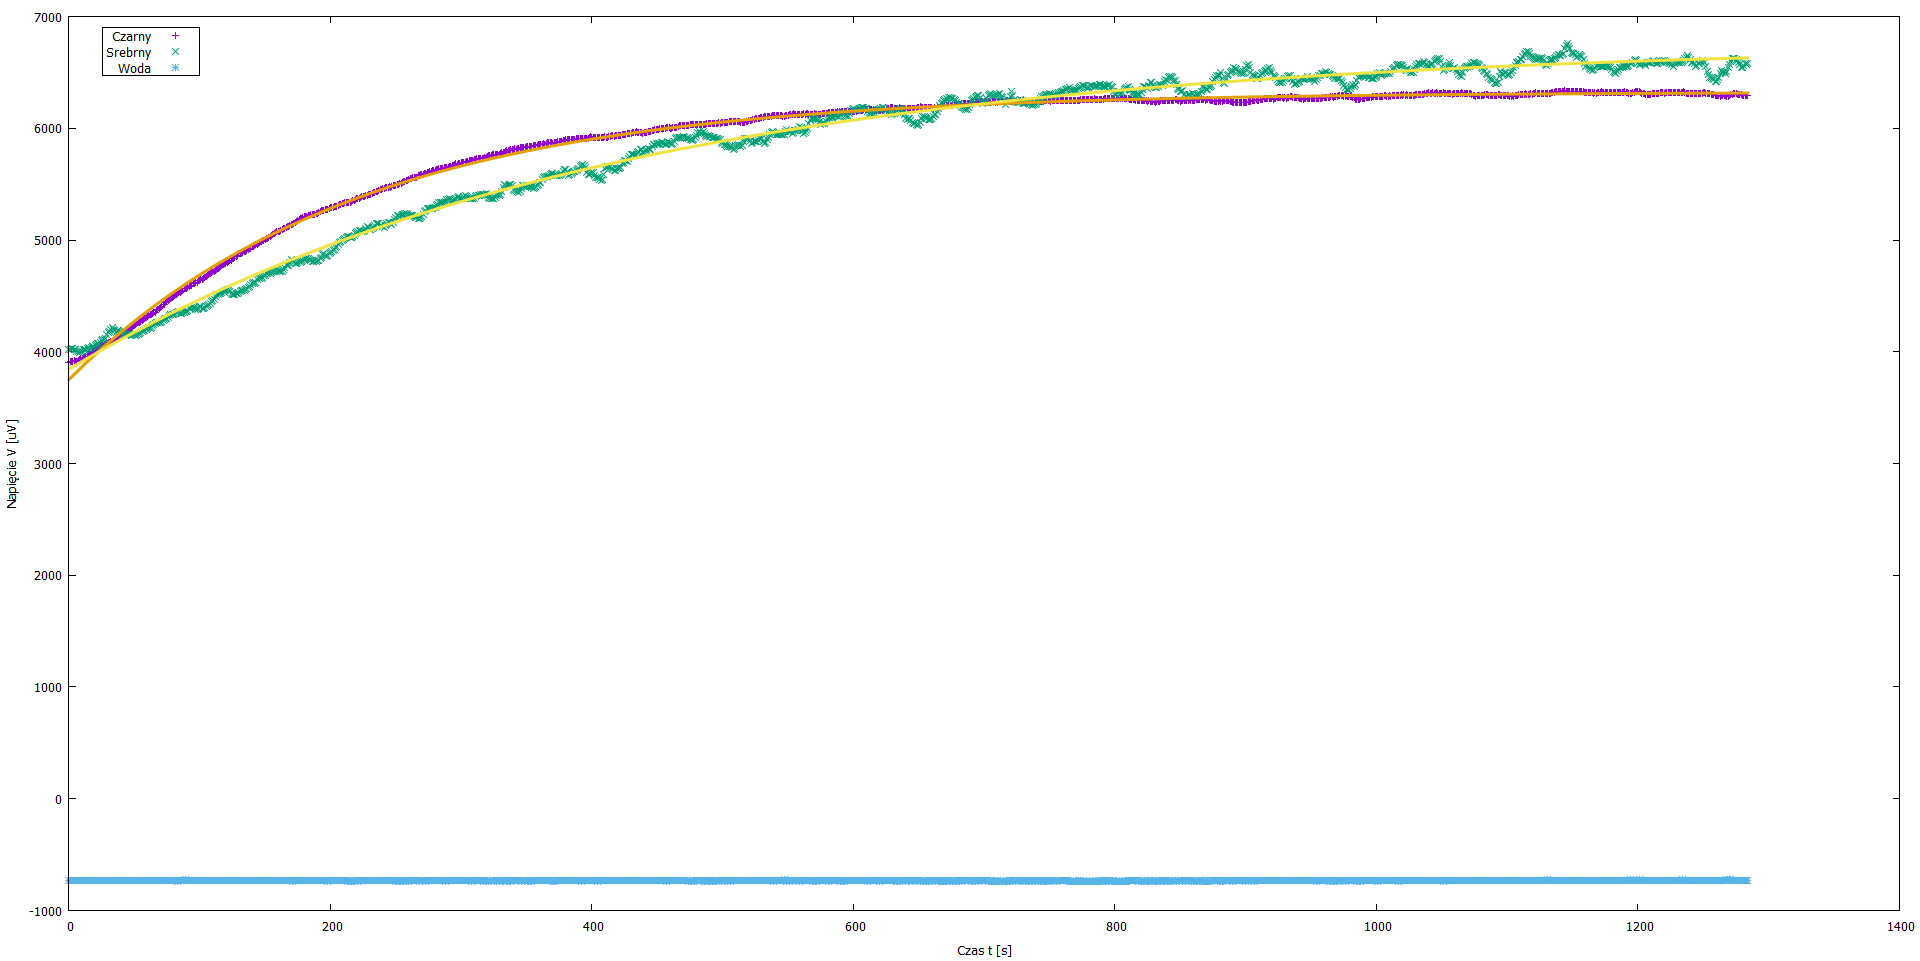
\includegraphics[width=8cm, height=5cm ]{rap11rys4} 
\caption{Dopasowanie krzywej: pomiar 3.}
\end{minipage}%
\begin{minipage}{0.5\textwidth}
  \centering
  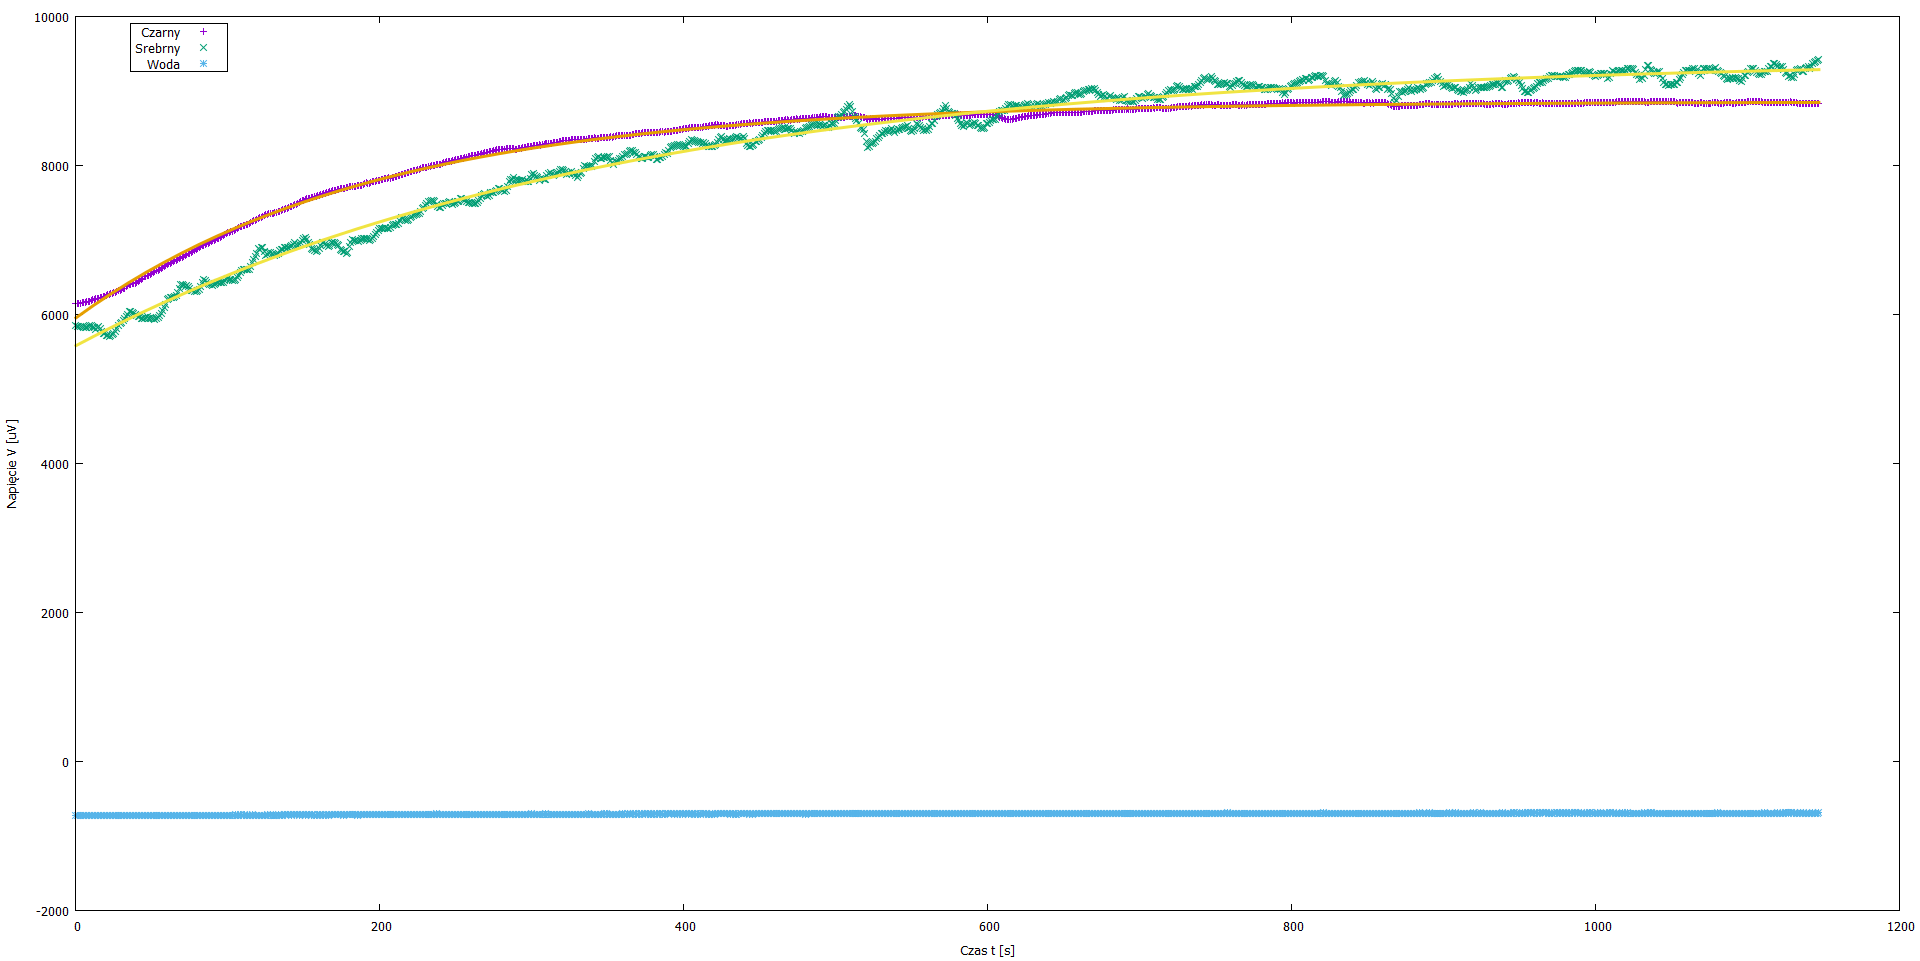
\includegraphics[width=8cm, height=5cm ]{rap11rys5} 
\caption{Dopasowanie krzywej: pomiar 4.}
\end{minipage}
\end{figure}
 

W Tabeli 3 zebrano wszystkie współczynniki wraz z ich niepewnościami.

\begin{table}[h!]
\centering
\caption{Wartości współczynników.}

\begin{tabular}{|c|c|c|c|c|}
\hline
\multicolumn{5}{|c|}{Walec czarny}                                     \\ \hline
\multicolumn{3}{|c|}{Pomiar 1}         & \multicolumn{2}{c|}{Pomiar 2} \\ \hline
Wielkość     & Wartość    & Niepewność & Wartość       & Niepewność    \\ \hline
$V_{\infty}$ [$\mu$V]& 2290,47    & 1,40       & 4186,94       & 2,003         \\ \hline
$V_{0}$ [$\mu$V]      & 2488,31    & 2,22       & 2255,33       & 3,503         \\ \hline
$\lambda$ [1/s]    & 0,00287143 & 0,0000067  & 0,003649      & 0,00001407    \\ \hline
$\chi^2$&\multicolumn{2}{c|}{13.76}	&	\multicolumn{2}{c|}{14,52}	 \\ \hline
\multicolumn{3}{|c|}{Pomiar 3}         & \multicolumn{2}{c|}{Pomiar 4} \\ \hline
$V_{\infty}$ [$\mu$V] & 6322,57    & 1,267      & 8854,56       & 1,676         \\ \hline
$V_{0}$ [$\mu$V]      & 2570,82    & 2,938      & 2899,77       & 4,194         \\ \hline
$\lambda$ [1/s]   & 0,00452882 & 0,000011   & 0,005123      & 0,000016      \\ \hline
$\chi^2$&\multicolumn{2}{c|}{6,04}	&	\multicolumn{2}{c|}{6,74}	 \\ \hline
\multicolumn{5}{|c|}{Walec srebrny}                                    \\ \hline
\multicolumn{3}{|c|}{Pomiar 1}         & \multicolumn{2}{c|}{Pomiar 2} \\ \hline
$V_{\infty}$ [$\mu$V] & 3007,66    & 2,549      & 4198,43       & 5,171         \\ \hline
$V_{0}$ [$\mu$V]      & 3197,05    & 2,616      & 2457,45       & 5,475         \\ \hline
$\lambda$  [1/s]  & 0,0020728  & 0,0000052  & 0,00253969    & 0,00001738    \\ \hline
$\chi^2$&\multicolumn{2}{c|}{18,26}	&	\multicolumn{2}{c|}{40,94}	 \\ \hline
\multicolumn{3}{|c|}{Pomiar 3}         & \multicolumn{2}{c|}{Pomiar 4} \\ \hline
$V_{\infty}$ [$\mu$V]& 6763,92  & 6,084    & 9438,89       & 9,727         \\ \hline
$V_{0}$ [$\mu$V]      & 2919,55  & 6,188    & 3857,2        & 10,17         \\ \hline
$\lambda$ [1/s]   & 0,002401 & 0,000016 & 0,002819      & 0,000023      \\ \hline
$\chi^2$&\multicolumn{2}{c|}{33,32}	&	\multicolumn{2}{c|}{56,23}	 \\ \hline
\end{tabular}
\end{table}

Na podstawie współczynników $V_{\infty}$ oraz Równania (3) i Równania (4) obliczono temperaturę walców wraz z niepewnościami. Wyniki przedstawiono w Tabeli 4.

\begin{table}[h!]
\centering
\caption{Temperatury walców.}
\begin{tabular}{|c|c|c|c|c|c|c|c|}
\hline
\multicolumn{4}{|c|}{Walec czarny}                             & \multicolumn{4}{c|}{Walec srebrny}                            \\ \hline
\multicolumn{2}{|c|}{Pomiar 1} & \multicolumn{2}{c|}{Pomiar 2} & \multicolumn{2}{c|}{Pomiar 1} & \multicolumn{2}{c|}{Pomiar 2} \\ \hline
T [$^{\circ}$C]      & $\Delta T$ [$^{\circ}$C]    & T [$^{\circ}$C]     & $\Delta T$ [$^{\circ}$C]    & T [$^{\circ}$C]     & $\Delta T$ [$^{\circ}$C]    & T [$^{\circ}$C]     & $\Delta T$ [K]    \\ \hline
71,71      & 0,86              & 113,00    & 1,07              & 87,55     & 0,94              & 113,25    & 1,07              \\ \hline
\multicolumn{2}{|c|}{Pomiar 3} & \multicolumn{2}{c|}{Pomiar 4} & \multicolumn{2}{c|}{Pomiar 3} & \multicolumn{2}{c|}{Pomiar 4} \\ \hline
157,26     & 1,29              & 206,65    & 1,53              & 166,11    & 1,33              & 217,57    & 1,59              \\ \hline
\end{tabular}
\end{table}

W ten sposób otrzymano możliwość powiązania mocy z temperaturą. Moc obliczono z klasycznego wzoru $W=IU$. Jednakże mierzone napięcie to napięcie na obu grzankach, więc otrzymana moc to łączna moc obu grzałek. Tak więc otrzymane wartości mocy należy podzielić na 2. Niepewność mocy obliczono metodą propagacji małych błędów. Ogólny wzór przenoszenia niepewności w tej metodzie jest następujący:

 \begin{equation}
 u_{f}^2=\sum_{i=1}^n \left( \dfrac{\partial f}{\partial x_{i}}u_{i}\right)^2+\sum_{i=1, i\neq j}^n \left( \dfrac{\partial f}{\partial x_{i}}\dfrac{\partial f}{\partial x_{j}}c_{ij}\right),
 \end{equation}
 gdzie wielkość $f$ zależy od wielkości $x_{i}$ o niepewnościach $u_{i}$ i o ocenach kowariancji $c_{ij}$ \cite{tay1}. W przypadku mierzonych napięć, kowariancja między nimi, a natężeniem wynosi 0. Ostatecznie niepewność mocy $W$ jest dana wzorem:
 \begin{equation}
 u_{W}=W\sqrt{\dfrac{u_{U}^2}{U^2}+\dfrac{u_{I}^2}{I^2}}
 \end{equation}

W Tabeli 5 przedstawiono wartości mocy na jednej grzałce oraz jej niepewność.

\begin{table}[h!]
\centering
\caption{Wartości mocy na grzałce.}
\begin{tabular}{|c|c|c|}
\hline
Pomiar & Moc W [W] & Niepewność $u_{W}$ [W] \\ \hline
1      & 3,61      & 0,17                   \\ \hline
2      & 7,23      & 0,30                   \\ \hline
3      & 12,10     & 0,49                   \\ \hline
4      & 18,23     & 0,70                   \\ \hline
\end{tabular}
\end{table}

Na potrzeby dalszej analizy postanowiono zamienić otrzymane wartości temperatury na temperaturę w kelwinach, poprzez dodanie doń wartości 273,15 K. Wykonano wykres $W(T)$. Jego wizualna analiza pozwoliła dostrzec, iż punkty układają się w kształt paraboli, jak i również to, iż punkt związany z trzecim pomiarem dla walca srebrnego znacząco odbiega od innych; jego wartość jest zbyt bliska wartości temperatury walca okopconego. Z tego powodu postanowiono odrzucić ten punkt w dalszej analizie. Dodano też punkt związany z temperaturą pokojową, który odpowiada zerowej różnicy emitowanej mocy. Do tych punktów dopasowano parabolę postaci:
\begin{equation}
W(T)=AT^2+BT+C.
\end{equation}

Rysunek 7 przedstawia punkty pomiarowe wraz z krzywymi dopasowania. Ze względu na to, że do punktów pomiarowych dodano stałą wartość z powodu zamiany skali temperatury, przeprowadzenie testu $\chi^2$ jest niemożliwe.


\begin{figure}[h!]
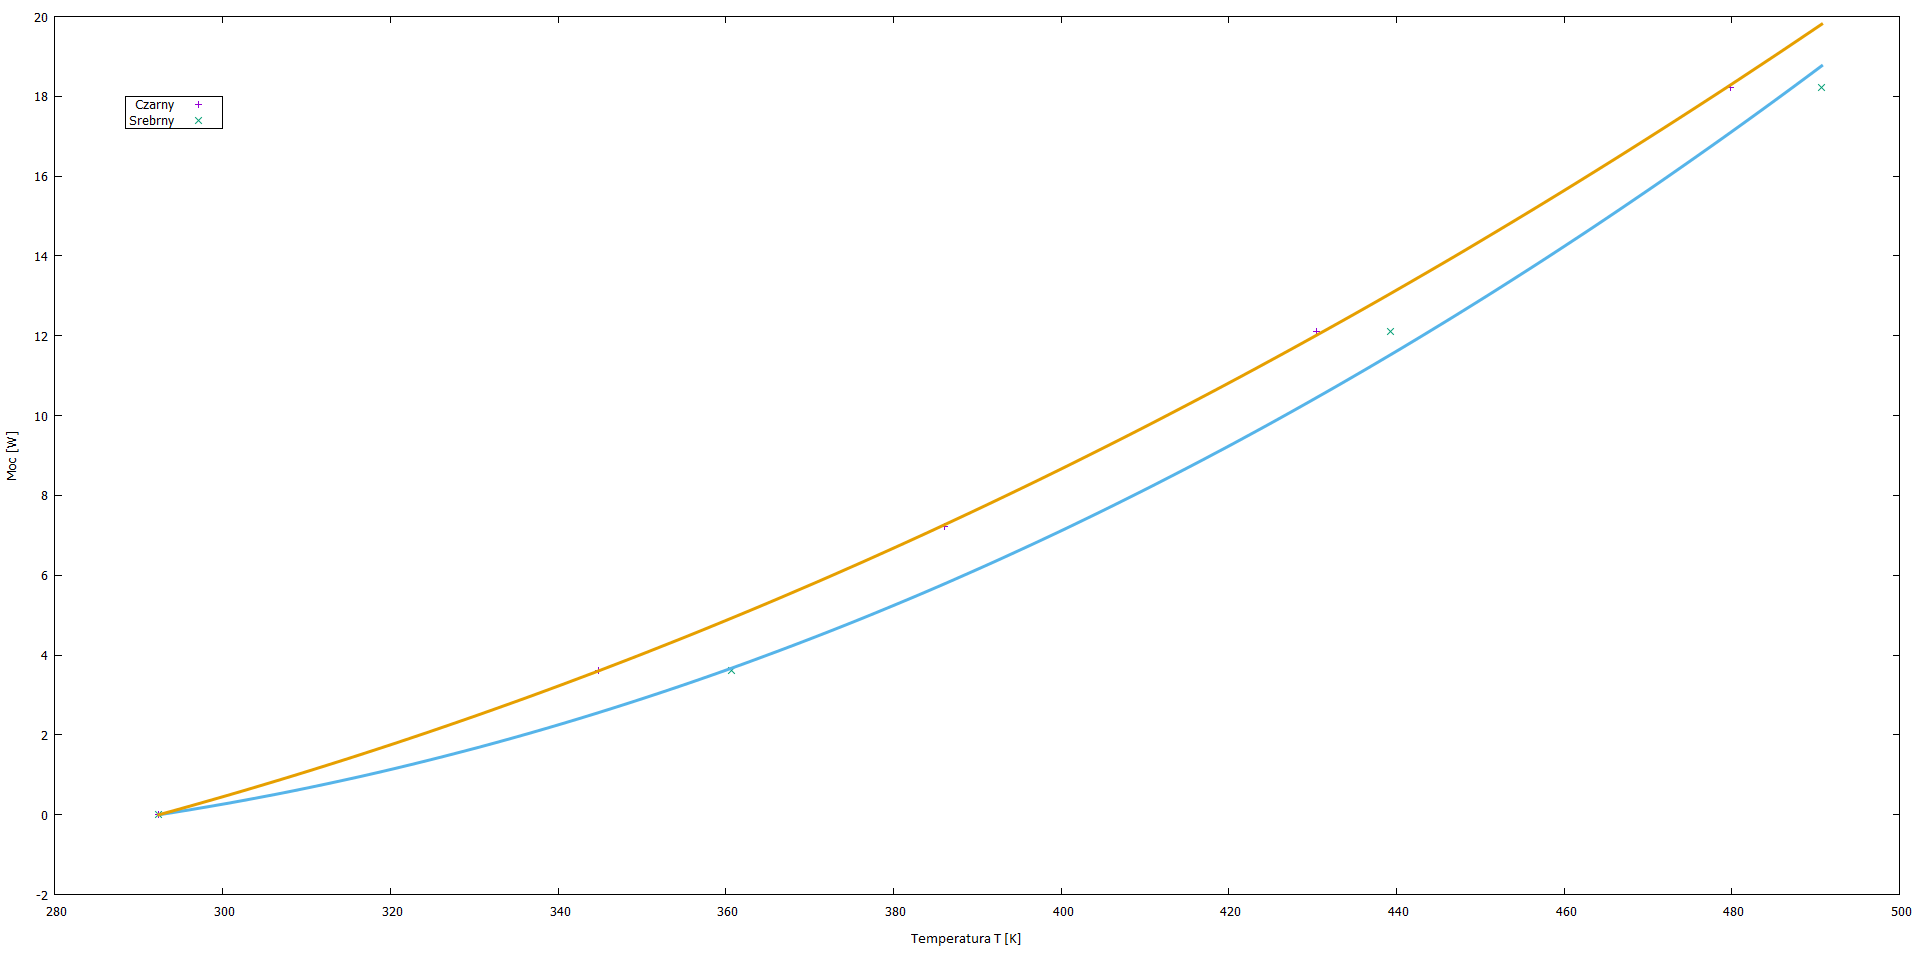
\includegraphics[width=15cm]{rap11rys6} 
\centering
\caption{Zależność mocy od temperatury.}
\end{figure}

Wartości współczynników dla obu parabol oraz oceny kowariancji $c_{ij}$ tych współczynników znajdują się w Tabeli 6. Poprzez $u_{i}$ oznaczono niepewność współczynnika $i$.

\begin{table}[h!]
\centering
\caption{Współczynniki parabol.}
\begin{tabular}{|c|c|c|c|c|c|c|c|c|c|}
\hline
Walec   & A  [W/K$^2$]        & $u_{A}$[W/K$^2$]   & B   [W/K]     & $u_{B}$[W/K] & C      [W] & $u_{C}$ [W]& $c_{AB}$ & $c_{AC}$ & $c_{BC}$ \\ \hline
Czarny  & 0,0002135  & 0,0000060 & -0,06733 & 0,0042  & 1,43233 & 0,71    & -0,998   & 0,993    & -0,999   \\ \hline
Srebrny & 0,00031408 & 0,000093  & -0,15136 & 0,0654  & 17,4035 & 11,19   & -0,998   & 0,993    & -0,999   \\ \hline
\end{tabular}
\end{table}

Teraz zyskano możliwość wyznaczenia funkcji różnicy mocy $\Delta W$. Uzyskano ją odejmując funkcję paraboliczną walca okopconego od funkcji walca wypolerowanego. Wyznaczono wartości różnicy funkcji dla temperatur z Tabeli 4 oraz dla temperatury pokojowej. Zgodnie z Równaniem (2) otrzymana zależność powinna być zależnością liniową dla czwartej potęgi temperatury. Otrzymane punkty, przedstawione w Tabeli 7, naniesiono na wykres przedstawiony na Rysunku 8.


\begin{table}[h!]
\centering
\caption{Różnica mocy.}
\begin{tabular}{|c|c|c|c|c|c|c|c|c|c|}
\hline
T [K]          & 292,40    & 344,86 & 386,15 & 430,41 & 479,80 & 360,70 & 386,40 & 439,26 & 490,72 \\ \hline
$u_{T}$ [K]    & 0,42      & 0,86   & 1,07   & 1,29   & 1,53   & 0,94   & 1,07   & 1,33   & 1,59   \\ \hline
$\Delta W$ [W] & -0,000026 & 1,046  & 1,480  & 1,564  & 1,193  & 1,253  & 1,481  & 1,534  & 1,044  \\ \hline
$u_{\Delta W}$ [W] & 0,034759  & 0,28   & 0,17   & 0,31   & 1,27   & 0,28   & 0,17   & 0,45   & 1,54   \\ \hline
\end{tabular}
\end{table}

\begin{figure}[h!]
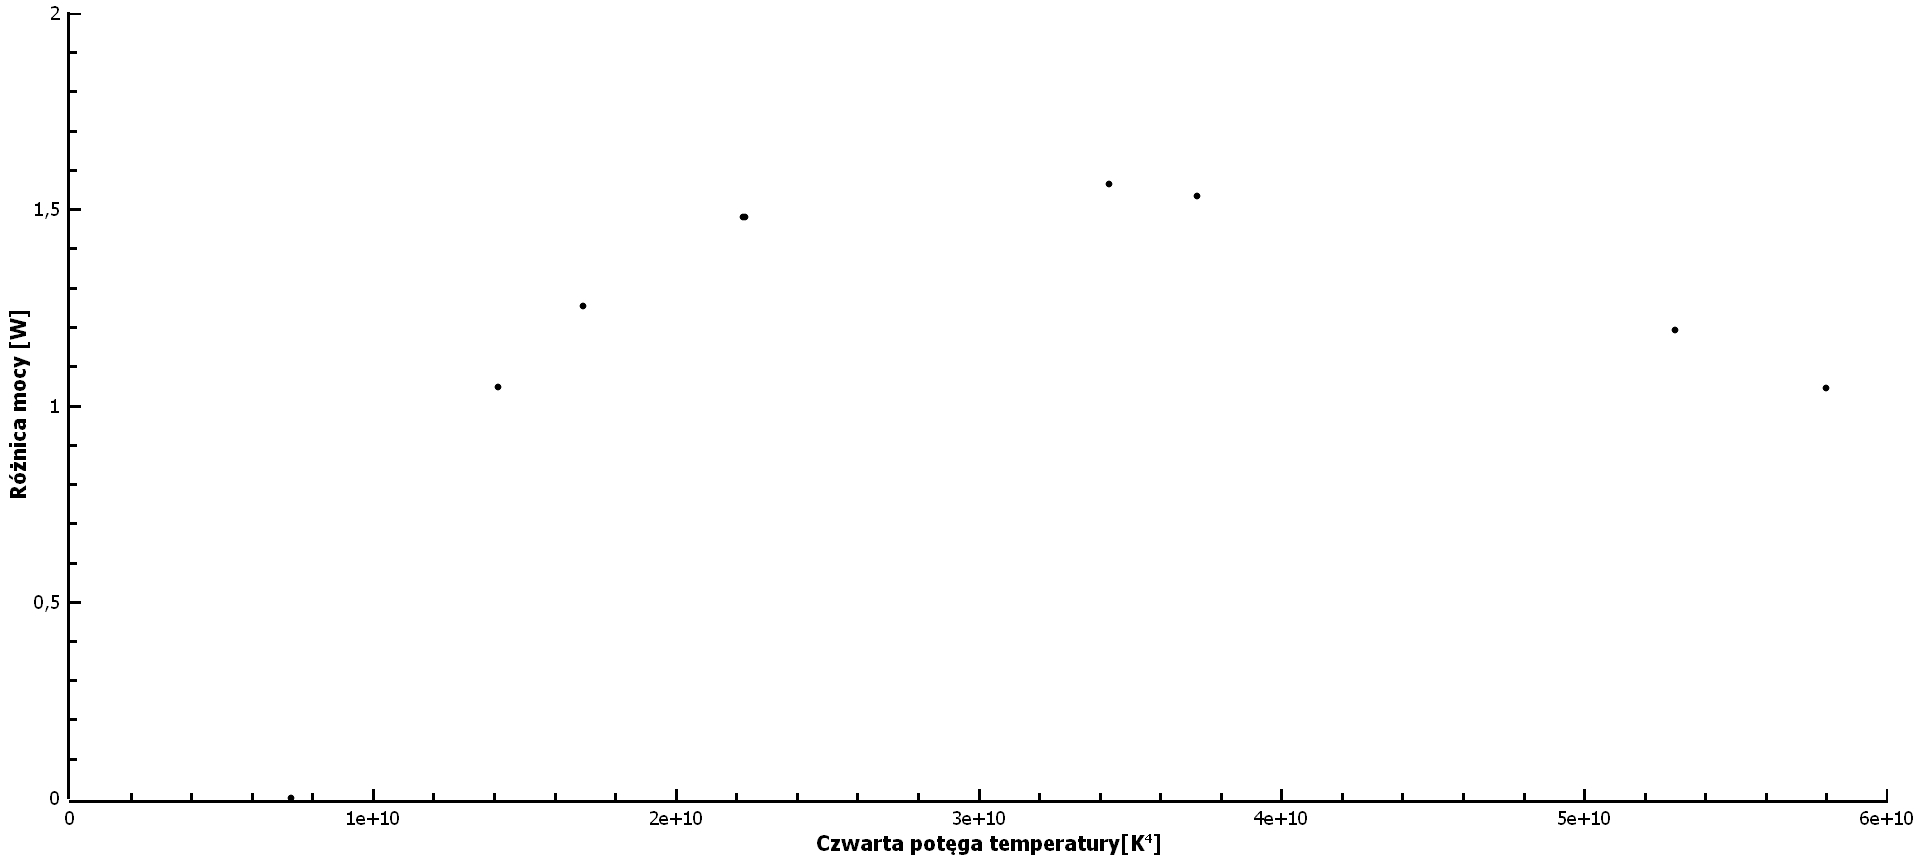
\includegraphics[width=15cm]{rap11rys7} 
\centering
\caption{Zależność różnicy mocy od temperatury.}
\end{figure}


Jak widać otrzymana zależność w niczym nie przypomina zależności liniowej. Można było to przewidzieć, analizując Rysunek 7, gdyż w rozpatrywanym przedziale różnica między funkcjami początkowo rośnie, a następnie zaczyna maleć. Z tego też powodu postanowiono odrzucić większość punktów i zachować tylko pierwsze cztery punkty, które wykazują zależność liniową. Niepewności tych punktów obliczono, korzystając z (9) wraz z uwzględnieniem kowariancji. Otrzymane wyniki wskazują na to, że względna niepewność różnicy mocy jest znacznie większa od względnej niepewności $T^4$, dlatego też w analizie danych, to temperatura będzie odkładana na osi OX. Dopasowanie danych przy pomocy Gnuplot do krzywej postaci $y=ax+b$ zwróciło wartości: $a=(8,1\pm1,8)\cdot10^{-11}$ W/K$^4$, $b=-0,58\pm0,17$ W. Krzywą wraz z punktami przedstawiono na Rysunku 9.

\begin{figure}[h!]
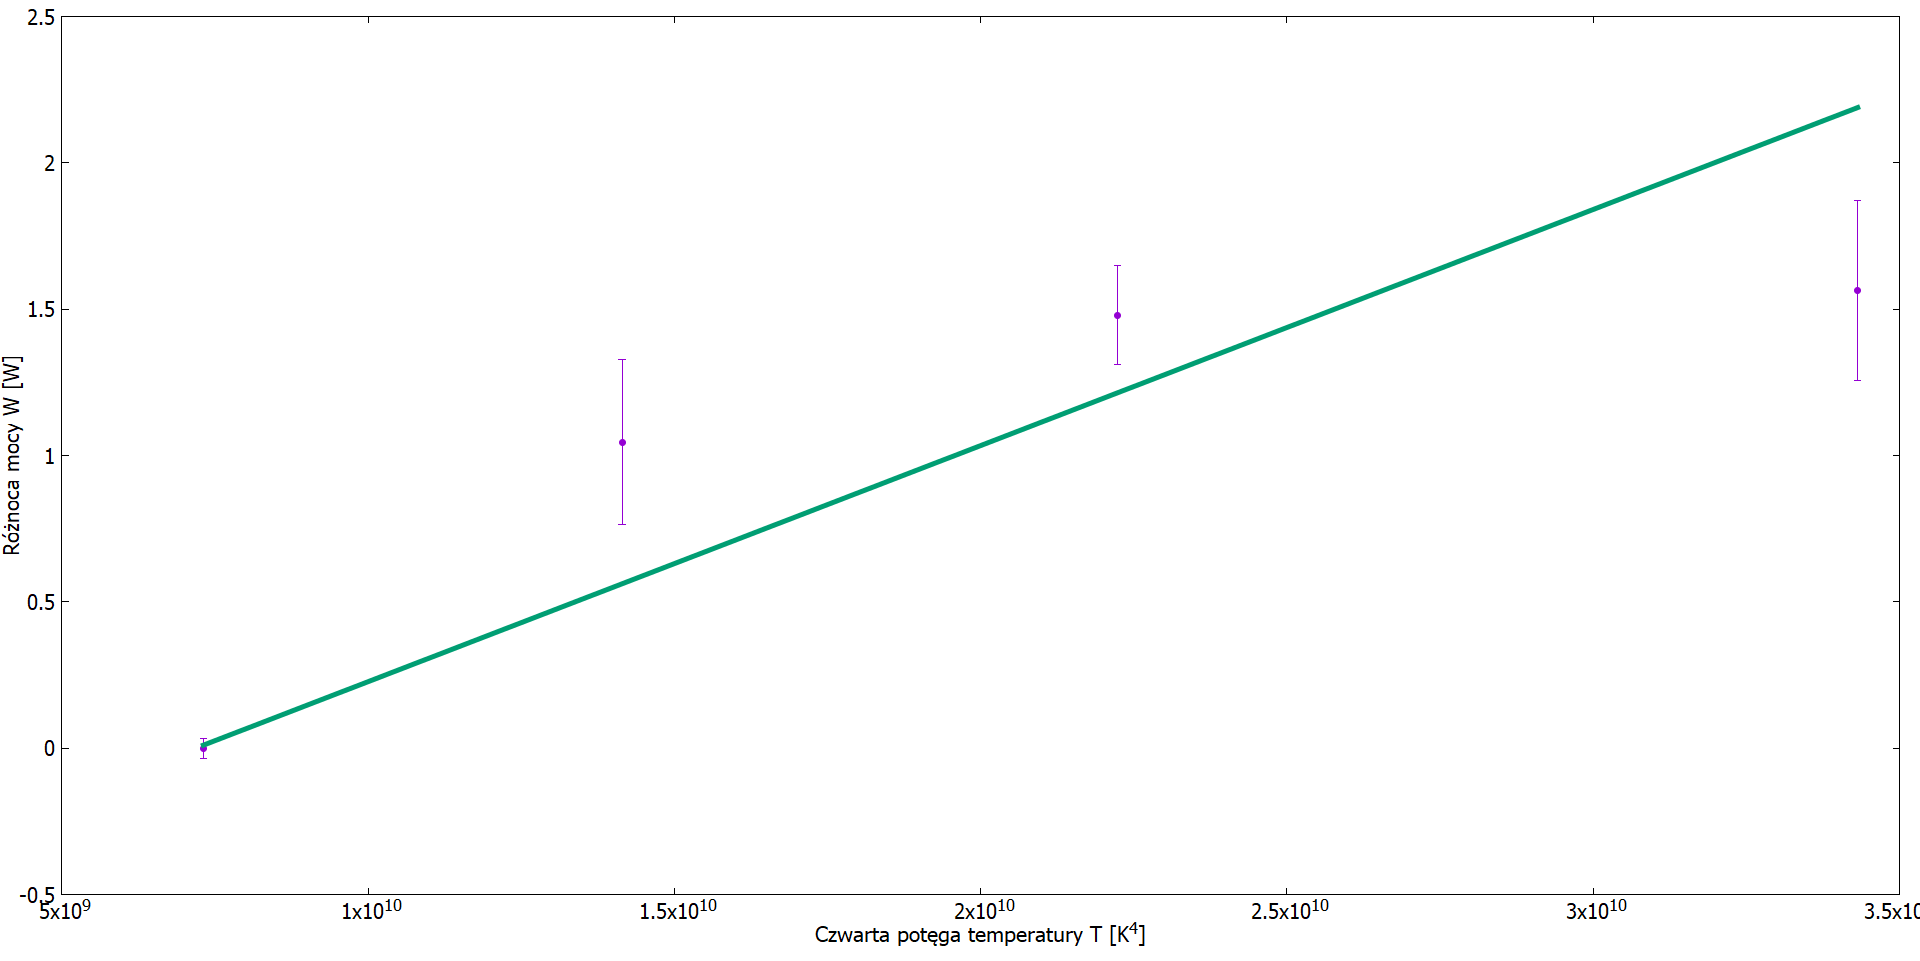
\includegraphics[width=15cm]{rap11rys8} 
\centering
\caption{Zależność różnicy mocy od temperatury.}
\end{figure}
Otrzymana wartość $\chi^2=4,83$ jest mniejsza od wartości krytycznej wynoszącej 5,99, tak więc krzywą można uznać za niesprzeczną z danymi.

Współczynnik $b$ jest wartością strat energii do otoczenia, a współczynnik $a$ odpowiada wielkości $(1-\epsilon)S\sigma$. Aby wyznaczyć wartość stałej Stefana-Boltzmanna konieczne jest jeszcze obliczenie pola walca. W tym celu uśredniono dane z Tabeli 2, za niepewność średnicy przyjęto wartość 0,1 mm, a za niepewność wysokości przyjęto wartość 1 mm. Wybrano takie niepewności, gdyż eksperyment zakłada identyczność walców, a takie niepewności sprawiają, że wszelakie różnic między ciałami mieszczą się w niepewnościach.
Niepewność pomiaru pola $S$ obliczono, korzystając z Równania (9). Otrzymano $S=3417\pm52$ mm$^2$. Wartość współczynnika $\epsilon$ wynosiła $0,06\pm0,01$. Korzystając z otrzymanych wartości oraz z Równania (9) wyznaczono wartość stałej Stefana-Boltzmanna $\sigma=(2,51\pm0,56)\cdot 10^{-8}$ W/m$^2$K$^4$. Otrzymana wartość jest dwukrotnie niższa od wartości teoretycznej, która wynosi $5,67\cdot 10^{-8}$. 

\begin{center}
\textbf{\subsection*{DYSKUSJA WYNIKÓW I WNIOSKI}}
\end{center} 
Otrzymana wartość, choć niższa od oczekiwanej, pozwala na poprawne oszacowanie rzędu wielkości szukanej stałej. Sama rozbieżność wyników wynika zapewne z faktu, iż termopara odpowiedzialna za pomiar napięć na walcu srebrnym nie była odpowiednio dobrze zamocowana, co powodowało jej wypadanie. Dodatkowo walce nie były idealnie osłonięte, co czyniło je wrażliwymi na prądy powietrza. Kumulacja tych niedogodności doprowadziła do rozbieżności wyników już na etapie pomiarów napięcia, co ostatecznie dało o sobie znać przy dopasowywaniu krzywej z Rysunku 8 i Rysunku 9. Sam Rysunek 9 daje jasno do zrozumienia, że dokładne wyznaczenie stałej było niemożliwe.

\begin{center}
\begin{thebibliography}{9}

\bibitem{tay1}
 J. R. Taylor,
 \emph{Wstęp do analizy błędu pomiarowego},
 PWN, Warszawa, 1995, s. 175.
 

 \end{thebibliography}

\end{center}


\end{document}